\documentclass[a4paper,8pt,twocolumn]{extarticle}
\usepackage[utf8]{inputenc}
\usepackage{graphicx}
\usepackage[center]{caption}
\usepackage[english]{babel}
% \usepackage[top=3cm, bottom=3cm, left=2cm, right=2cm]{geometry}

%---------------------------------------------
% Font packages
%---------------------------------------------
\usepackage{lmodern}
% \usepackage{concmath}
% \usepackage{cmbright}
% \usepackage{kpfonts}
% \usepackage[adobe-utopia]{mathdesign}
% \usepackage{fouriernc}
\usepackage[T1]{fontenc}

%---------------------------------------------
% Math environment packages & command
%---------------------------------------------
\usepackage{amsmath}
\usepackage{amssymb}
\usepackage{array}
% \usepackage{mathrsfs}
\usepackage{array}
% \def\sgn{\mathop{\rm sgn}\nolimits} 
% \usepackage{bbm}


%---------------------------------------------
% item option
%---------------------------------------------
\renewcommand{\labelitemi}{-}


%---------------------------------------------
%HEADER & FOOTER
%---------------------------------------------
\usepackage{fancyhdr}
\pagestyle{fancy}

\renewcommand{\headrulewidth}{.15pt}
\fancyhead[C]{{\textsc{The Guarding Problem}}} 
\fancyhead[L]{Page \thepage \ of \pageref{LastPage}}
\fancyhead[R]{DD2438}

\renewcommand{\footrulewidth}{.15pt}
\fancyfoot[C]{\thepage} 
% \fancyfoot[L]{truc}
% \fancyfoot[R]{bidule}

\usepackage{lastpage}

%---------------------------------------------
% two column option
%---------------------------------------------
\setlength{\columnsep}{0.7cm}

%---------------------------------------------
% Table of content
%---------------------------------------------
\usepackage[colorlinks,linkcolor=black, citecolor=black]{hyperref}

%---------------------------------------------
% Opening
%---------------------------------------------
\title{Artificial Intelligence \& Multi-Agent System :\\ \textsc{The Guarding Problem}}
\author{Björn \textsc{Holm}, Kilian \textsc{Demeulemeester} \\ \texttt{\{bjh,kiliande\}@kth.se}}

%---------------------------------------------
% Numerotation Handling
%---------------------------------------------
 %\setcounter{section}{3}
 \usepackage[explicit]{titlesec}
  %\titleformat{<command>}[<shape>]{<format>}{<label>}{<sep>}{<before>}[<after>]
	\titleformat{\section}[block]{\Large\bfseries\filcenter}{\arabic{section}.}{1em}{#1}
 %\titleformat{\section}[hang]{\normalfont\Large\bfseries}%
     %{}{8pt}%
     %{\arabic{section}. #1}



%---------------------------------------------
% Dummy text
%---------------------------------------------
\usepackage{lipsum}

%---------------------------------------------
% Enumeration spacing
%---------------------------------------------
\usepackage{enumitem}
\setlist[enumerate]{itemsep=0mm}
\setlist[description]{itemsep=0mm}

%---------------------------------------------
% Algorithm form
%---------------------------------------------
\newtheorem{algorithm}{Algorithm}[section]
\newtheorem{criteria}{Criteria}[section]
\newtheorem{problem}{Problem}
    
\begin{document}

% Indentation size
%\setlength\parindent{0em}

 \maketitle

\tableofcontents

\vspace{0.5cm}
\hrule
\vspace{0.5cm}

\begin{bfseries}
\emph{Abstract} -- 
The purpose of this project was to create an environment -- using \texttt{Unity} -- where vehicules execute cooperativly search and pursuit of intruders. The problem involves optimising different algorithms such as discretizing an environment, computing a minimal path for a fleet of vehicule that are to survey a given area, optimizing the search of a mobile intruder, pursuiting and capturing an intruder.

In this paper we focus on three different problems. The first is how to find the position of static guards such that a given set of building is completly guard. The second problem is how to clean a area with moving guard -- \emph{i.e.} every part of the area has been seen. The third problem is how to search and capture a moving intruder that is trying to escape.
\end{bfseries}


\section{The three problems}
Our work was divided into three main problems, even if we tried to keep a high level of generality in order to use as much as possible the different algorithm in the three of them.

\begin{problem}[Static Guarding]
Given an area with obstacles, find a set of point $P_{1\leq i \leq n}$ such as every free point of the area is seen from a least one $P_i$, with $n$ as small as possible. It is also referred as the art gallery problem.
\end{problem}
\begin{problem}[Dynamic Guarding]
Given an area with obstacles, find paths for $n$ robot ($n$ is a parameter) in order to clear the whole area (\emph{i.e} Each point of the area has been seen).
\end{problem}
\begin{problem}[Search \& Capture]
Given an area, find paths for $n$ robot ($n$ as small as possible) in order to find a moving intruder. Once it is located, pursue him in order to capture him.
\end{problem}

\section{Environment representation}
For all the problems dealt with in this report, the environment is represented as a two dimensional polygon with holes. However, we restrict ourselves to only deal with environments with orthogonal, i.e. only consisting of horizontal and vertical lines. With another algorithm for tesselating the environment the other algorithms could work for any polygonal environment.

In order to enhance the performance, we discretize our environment using a grid. Each cell is either \emph{occupied} if one of its corners lies into an obstacle or \emph{free}.
The environment is then tesselated into convex areas, we use rectangles, $C_{1\leq i \leq n}$ each satisfying the following criteria.

\begin{criteria}[of Visibility]
 \emph{For all point $P$ in the environment, if each corner of $C_i$ is visible, then $C_i$ is completely visible}. In practice, it means that checking if a area is completely visible from a given point can be done in only 4 raycasts (because a rectangle has 4 corners).
\label{visibilityCriteria}
\end{criteria}


The three problems we investigate involve finding interesting points on the map. We use the following terminology:
\begin{definition}[Points of surveillance:]
All the points from which a specific area is completely visible.
\end{definition}

\subsection{Convex tesselation}

In order to solve our three problems, we need a convex tesselation of our environment. The algorithm used to create the convex tesselation is based on the work from \cite{CoopMinTime}. Figure \ref{convexTesselation} shows the convex tesselation generated by the algorithm \ref{algoConvexTesselation}.

\begin{algorithm}
This algorithm describes how to create a convex tesselation of our environment. Since the obstacles are all orthogonal, we construct our convex tesselation as rectangles aligned with the polygons.
\begin{enumerate}
\item Based on the grid, make a discretization of the environment $G(A)$.
\item Find a yet uncovered cell, $p$.
\item Start growing a rectange $C_i$ from $p$ until its length and width reach $R$\footnote{R is the maximum convex size in width and/or length. This parameter is used to guarantee the visibily criteria \ref{visibilityCriteria}}.
\item While uncovered cells exists, goto 2.
\end{enumerate}
\label{algoConvexTesselation}
\end{algorithm}

\subsection{Graph representation \& search}
\begin{definition}[Waypoint]
Point at a given distance from an obstacle's corner (see Figure \ref{waypointNavigation}).
\end{definition}
For guard navigation in the environment, we perform an A*-search on the connectivity graph between the waypoints, also including the starting position and the goal position.


\section{Static Guarding}
This problem is solved using the greedy algorithm \ref{algStaticGuard}, which generate a set of point $ S = P_{1\leq i \leq n}$ from which the environment is completely visible. Figure \ref{convexTesselation} shows the set of points produced by the algorithm.

\begin{algorithm}
This algorithm gives a way to find a set of points from which the environment is completely visible.
\begin{enumerate}
	\item Generate a set of potential points (we used the center of every grid cell).
	\item Create a set of unseen areas $U_i = C_i$ (see alg. \ref{algoConvexTesselation}).
	\item Find the point $p$ from which most of the area is visible.
	\item Add this point to the set of point $S$.
	\item Remove areas visible from $p$ from $U$.
	\item While there are unseen areas left, go to 3.
\end{enumerate}
\qed
\label{algStaticGuard}
\end{algorithm}

Even if there is no guarantee that algorithm \ref{algStaticGuard} will find the optimal solution, its low complexity ($\mathcal{O}(n)$ -- where $n$ is the size of the set) has been proven to be the best-possible polynomial time approximation algorithm for set cover (see \cite{approxMinProb}).

\begin{figure}[h!t]
	\begin{center}
	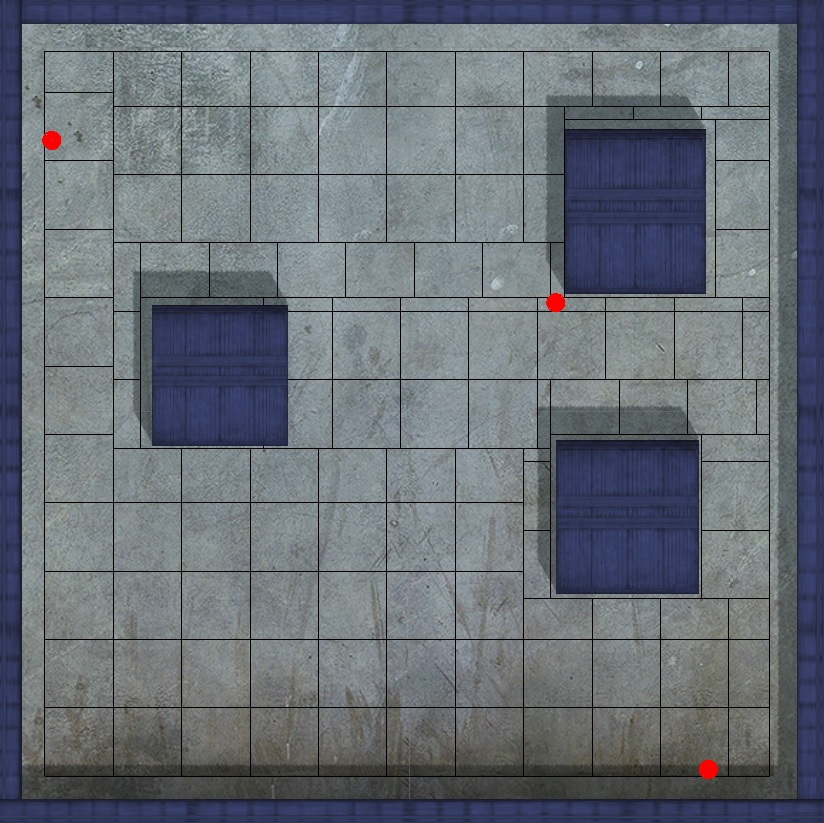
\includegraphics[width=\linewidth,natwidth=824,natheight=823]{fig/staticCoverSet.jpg}
	\end{center}
	\caption{Set cover \& Positions for static guarding}
	\label{convexTesselation}
\end{figure}


\section{Dynamic Guarding}
This problem is solved using the set of point $S$ produced by the algorithm \ref{algStaticGuard}. Based on the knowledge of this points, clearing the whole area can be done easily. It is enough to have each guard visiting once each of this points to guarantee that there is no static intruder (since the whole area will be seen). Figure \ref{dynamicPath} shows the paths for 4 vehicles cleaning an area.

The problem can then be stated as the following:

\begin{subproblem}
 Knowing the set of point $S$ and with a given number $n_{G}$ of guard, find the minimum path for each guard with the following condition:
 \begin{itemize}
  \item Each point has been seen once,
  \item The time to visit each point of $S$ is the smallest possible.
 \end{itemize}
This problem is quiet similar to the vehicles routing problem.
\label{subProb3}
\end{subproblem}

\subsection{Problem modelization}

The problem is modelize as the following:

\begin{enumerate}
  \item Create a matrix \textbf{Cost} with $\text{\textbf{Cost}}_{i,j} = \text{Length}(P_i,P_j)$ (real path length).
  \item Index each point of $S$ from $1$ to $n_{S}$.
  \item Index each guard from $n_{S}+1$ to $ n_{S}+n_{G}$.
  \item Each permutation $\sigma$ of $\{1,\hdots,n_{S}+n_{G}\}$ is a potential solution if $\sigma$ satisfy criteria \ref{permCriteria}
  \item $Cost(\sigma_1) \leq Cost(\sigma_2) \Longleftrightarrow$ $$\max_{k,\sigma_1}\text{PathLength}(\text{Guard}_k) \leq \max_{k,\sigma_2}\text{PathLength}(\text{Guard}_k)$$
  (It means that we will look for the solution where the guards have the smallest path possible.)
\end{enumerate}

\begin{criteria}
 Given a set $S$ of $n_S$ points and $n_G$ guards, a permutation $\sigma$ of $\{1,\hdots,n_S+n_G\}$ is valid if each $\sigma_i \in \sigma$ has a predecessor stricly bigger than $n_S$  -- it means that each point is visited once.
 \label{permCriteria}
\end{criteria}


\subsection{Exhaustive search}

Algorithm \ref{algExhDynamic} is testing every permutation of $\{1,\hdots,n_{S}+n_{G}\}$, but rapidly check if a permutation is a real potential solution, getting rid of a maximum of them. This algorithm performed well for small value of $n_S + n_G$ (until $\approx 10$).

\begin{algorithm}
This algorithm gives a way to find the smallest path for a set of $n_{G}$ vehicle to visit a set $S = P_{1\leq i \leq n_S}$ of point.
\begin{enumerate}
  \item Generate a valid permutation of $\{1,\hdots,n_{S}+n_{G}\}$.
  \item If each indices in $\{n_S +1, \hdots , nS +nG\}$ are in ascending order and if each robot visit a maximum of $\left \lceil{\frac{n_P}{n_G}}\right \rceil$ (ceil function)
  \begin{enumerate}
  \item Compute the total length represented by the permutation using the matrix \textbf{Cost}.
  \item Keep this permutation in memory if its the best so far.
  \end{enumerate}
\item While there is valid permutations go to 1.
\end{enumerate}
\qed
\label{algExhDynamic}
\end{algorithm}


\subsection{Tabu search}

Algorithm \ref{algExhDynamic} has a upper limit of $10$ since its checking every possible permutation. We need to be able to explore bigger environment -- more points to explore and/or more guards. In order to do so, we implemented a tabu--search like algorithm. Its performances are more than decent and its computational time is \emph{almost} constant, providing a solution close to the optimal one.

It is needed to understand the following notion before reading algorithm \ref{algExhDynamic}:
\begin{description}
 \item[Tabu-list:] List of fixed size with a storage of the permutation already processed in the close past.
 \item[Diversification:] If the algorithm is stuck in a local minima, diversification is needed. To do so, we generate a random valid permutation and start our search from there
 \item[Neighbourood:] Given a permutation $\sigma$, its neighbourood is defined has the permutations than can be reached from $\sigma$ by applying a swap of two adjacent index ($i \leftrightarrow i+1$) or a swap of 4 adjacents number ($(i,i+1) \leftrightarrow (i+2,i+3)$)
\end{description}


\begin{algorithm}
  This algorithm provide a way to find a ``close to optimal'' solution of problem \ref{subProb3} 
  \begin{enumerate}
   \item Generate a random valid permutation $\sigma_{best}$.
   \item Generate all the valid permutations in the \textbf{neighbourood} of $\sigma_{best}$.
   \item Foreach $\sigma_{potential}$ in this \textbf{neighbourood}
   \begin{enumerate}
    \item If $\sigma_{potential}$ is not in the tabu-list
    \begin{enumerate}
     \item Check if its a better solution than $\sigma_{best}$ (and eventually replace it)
     \end{enumerate}
   \end{enumerate}
     \item Add $\sigma_{best}$ to the tabu-list.
     \item If the solution has not improved since a given number of step, apply \textbf{diversification}.
   \item While the maximum of step has not been reached, go to 2. 
  \end{enumerate}
   \qed
 \label{tabuSearchAlg}
\end{algorithm}

In our case, algorithm \ref{tabuSearchAlg} has proved itself good with the following parameters:
\begin{itemize}
 \item 10.000 steps
 \item Diversification after 20 steps with no improvement
 \item Tabu-list of size 100
\end{itemize}




\begin{figure}[h!t]
	\begin{center}
	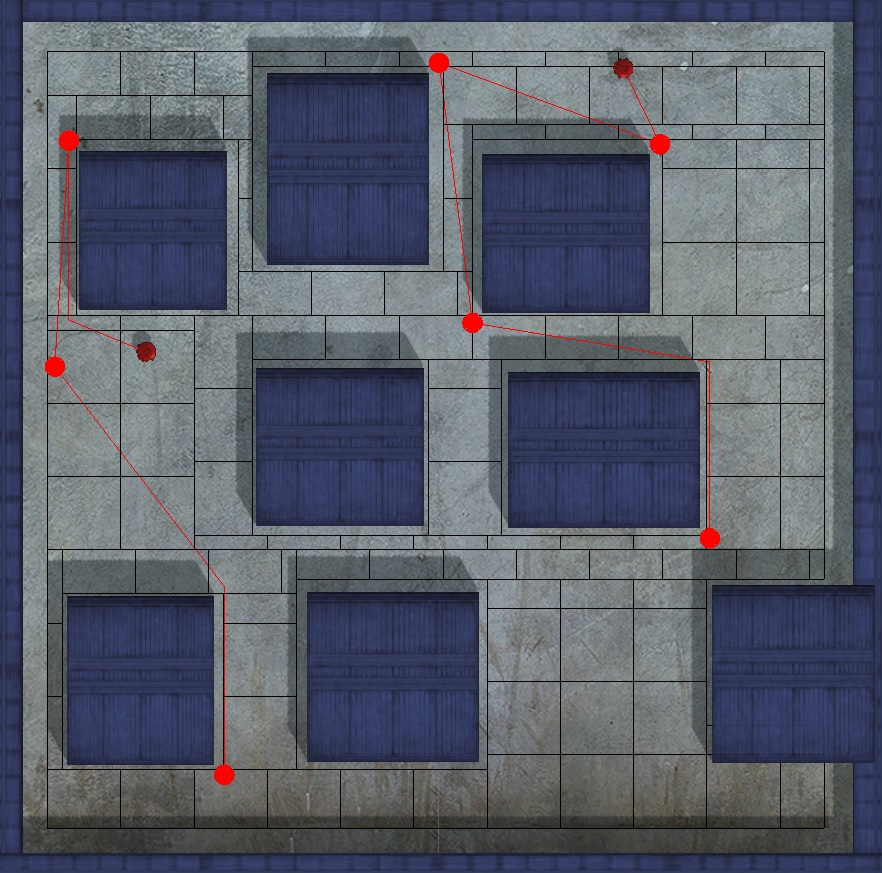
\includegraphics[width=150px]{fig/dynamicPath.jpg}
	\end{center}
	\caption{Path for $4$ vehicles looking for a static intruder}
	\label{dynamicPath}
\end{figure}





\section{Search \& Destroy}
We only have an idea for an algorithm for solving this problem, it is not yet tested.

The algorithm is based on ref\{one of P. Ögren's papers\} and the basic idea is to first place robots to break the problem down into smaller problems until a single robot can completely secure the smaller problem.
Once an area has been secured, it should never be allowed to be directly connected to unsecured areas again.
After securing, again try to break down the remaining problem into smaller problems and recurse.\\

Each area has two different boolean properties:
\begin{definition}[Watched]
if at least one robot can see the whole area.
\end{definition}
\begin{definition}[Secured]
if all of it's neighbors are either secured or watched.
\end{definition}

Each robot only has one property:
\begin{definition}[Occupied]
if it is the only robot watching an area that is not secured itself, but connected to both secured and unsecured areas.
\end{definition}

\begin{algorithm}
This is an algorithm for finding the points for robots to visit in order to secure a given 2D vector environment divided into free-space and obstacles. Intruders are allowed to move arbitrarily fast.

The algorithm is greedy, but corresponding versions of searching for and evaluating different solutions could also be made.
\begin{enumerate}
	\item Tesselate the environment into convex polygons and generate a graph of the connected polygons. (see Figure \ref{searchDestroy})
	\item Somehow find a point $p$ which divides the graph into smaller graphs. (see Figure \ref{searchDestroy2})
			Preferably, at least one of the smaller graphs should be of a size smaller than the number of currently available unoccupied robots.
	\item Move an unoccupied robot to $p$, if all robots are occupied, add a new robot at $p$.
	\item If all the areas are either secured or watched, we are done, otherwise, goto 2.
\end{enumerate}
\label{algSearchDestroyIdea}
\end{algorithm}

The possible points to visit and how placing a robot at that point transforms the graph could possibly be pre-generated.

\begin{figure}[h!t]
% 	\includegraphics[width=0.1\linewidth, height=0.1\linewidth]{fig/searchdestroy.png}
	\caption{The tesselation (red) and graph (black) of an environment}
	\label{searchDestroy}
\end{figure}

\begin{figure}[h!t]
% 	\includegraphics[width=\linewidth, height=\linewidth]{fig/searchdestroy.png}
	\caption{TODO: the new graph after placing a robot at a point}
	\label{searchDestroy2}
\end{figure}


\section*{Conclusion}
\addcontentsline{toc}{section}{Conclusion}
We have in this report described how we solved the problems of finding a static surveillance (the art gallery problem) and finding patrol paths for moving guards looking for immobile intruders.
We have also given an idea for an algorithm to secure an environment while the intruders are moving around.

None of our solutions are guaranteed to be optimal, but visual inspection suggests them to be quite good.


\nocite{*}
\bibliographystyle{plain}
\bibliography{bibliography}

\end{document}
